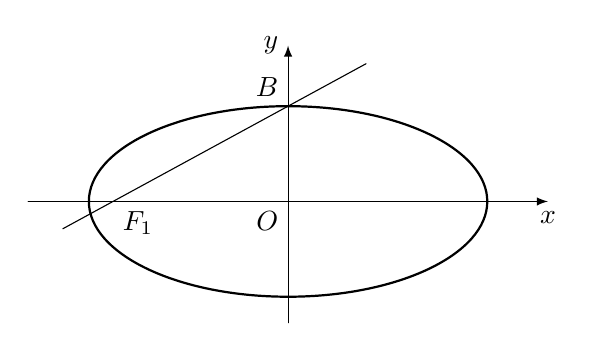
\begin{tikzpicture}[>=latex, scale=1.1, line join=round, line cap=round]
  % Axes
  \draw[->] (-3.0, 0) -- (3.0, 0) node[below] {$x$};
  \draw[->] (0, -1.4) -- (0, 1.8) node[left] {$y$};
  \node[below left] at (0, 0) {$O$};

  % Ellipse
  \draw[thick] (0, 0) ellipse (2.3 and 1.1);

  % Points
  \coordinate (F1) at (-2.02, 0);
  \coordinate (B) at (0, 1.1);

  % Line through F1 and B
  \draw (-2.6, -0.315) -- (0.9, 1.59);

  % Labels
  \node[below right] at (F1) {$F_1$};
  \node[above left] at (B) {$B$};
\end{tikzpicture}
